\documentclass{article}
\usepackage{comment}
\usepackage{graphicx}
\usepackage[utf8]{inputenc}
\usepackage[english]{babel}

\begin{document}

\title{Using wavelengths outside of the Telecom spectrum}
\author{Stefan Plug\\Remy de Boer}
\date{\today}
\maketitle

\begin{comment}
\begin{tabular}{|c|c|c|}
\hline 
Version number & Date & Comment \\ 
\hline 
0.1 & 03-01-2013 & Start of of document \\ 
\hline 
\end{tabular} 
\end{comment}

\tableofcontents
\newpage

\section{Preface}
\newpage
\section{Summary}
\newpage
\section{Research question}
It is common practice today to use Wavelength Division Multiplexing, WDM, devices on network links to increase the total amount of bandwidth that a single optical network link can carry. The WDM accomplishes this by assigning each input data stream its own unique light wavelength channel, $\lambda$. 
Not every wavelength is suitable for heavy traffic usage because of the physical characteristics of these channels. Our hypothesis is that these channels could be used for lower speed applications such as monitoring and out of band management.

To test our hypothesis we will look at the possibilities of the unused wavelengths outside of the Telecom spectrum.
The main research question will be as follows:
\begin{quote}
\textit{
What applications can the unused wavelengths outside of the Telecom spectrum be used for?
}
\end{quote}

It is important to be able to have an active monitoring system in place which can send out warnings when it detects either degradation of the link over time or a sudden change in the links characteristics, for example when someone places a tap on the link. 

To help us understand how we can effectively monitor an optical link we will ask the following sub-question:
\begin{quote}
\textit{
What optical link characteristics should we monitor?
}
\end{quote}

It could happen that the main traffic interface on a switch shuts down which could potentially shut down that section of the network.
It would be good to have a separate out of band network link up on another interface which could be used to still manage that device.

During this project we will focus on link monitoring and out of band management, but other usages may arise during our research.
If this should happen we shall try to document them.

\newpage
\section{Fibre Technology}
In this chapter we will elaborate on some of the used technology and techniques used for this research project.
\subsection{Fibreglass cables}
When using fibreglass networks, multiple types of fibreglass cables are used.
The two main categories used in computer networking are multi-mode and single-mode cables.
Multi-mode cables differ from single-mode cables as they consist of a larger core, which allows for easier connections and cheaper light sources such as LEDs. \cite{Fundamentals:2008}
For our projects we are focussing on single-mode cables, as these are the cables used with Wavelength Division Multiplexing (WDM).

\subsection{Wavelength division multiplexing}
Wavelength division multiplexing is a technique used to send multiple independent signals across the same fibre.
WDM works by combining optical signals of different wavelengths into a single fibre to increase the maximum bandwidth of a fibreglass cabl, thus allowing multiple completely separate connections to run along a single fibre cablee.
On either end of the single fibre cable, the signals are split into individual fibre cables and connected to their final destinations.

This ITU-T standard shows us that the 1625nm channel which resides at the beginning of the L-band is not officially supported by several of the single-mode optical cable standards as show in table \ref{tab:single-mode_types}.

\begin{table}[h]
\centering
\label{tab:single-mode_types}
\caption{ITU-T Single-mode cable standards}
\begin{tabular}{|c|c|c|}
\hline 
ITU-T code & Wavelength coverage\\ 
\hline 
G.652.A & O and C bands \\ 
\hline
G.652.B & O and C+L bands \\
\hline
G.652.C & From O to C bands \\
\hline
G.652.D & From O to L bands \\
\hline
\end{tabular} 
\end{table}

The cables which do not officially support the 1625nm channel are expected to generate a higher attenuation effect. Although we will not try to test this effect for all the different kinds of fibre, we should keep this in mind during testing.

\newpage
\section{Solution proof of concept}
\begin{figure}
\centerline{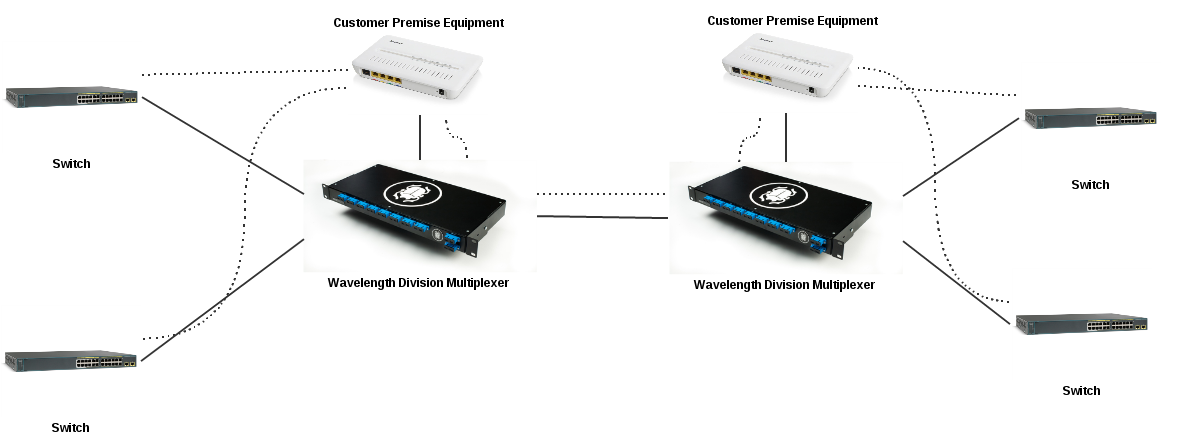
\includegraphics[scale=0.4]{images/rp1-monitoring-links.png}}
\caption{Network diagram of test setup}
\end{figure}

To test our hypotheses we built a proof-of-concept, consisting of the following components:
Test systems: 
\begin{itemize}
\item Inteno XG6746 \cite{Inteno:XG6746}
\begin{itemize}
\item Broadcom 6338
\item Marvell 88E6161
\item 8 MB Flash
\item 32 MB RAM
\end{itemize}

%\item Inteno EG500-R1 \cite{Inteno:EG500}
%\begin{itemize}
%\item Broadcom 6818
%\item 16 MB Flash
%\item 64 MB RAM
%\end{itemize}

\item Raspberry Pi - Model B

\item Optics:
\begin{itemize}
\item SFP
\item EOptolink
\item EOLS-1603-29SD
\item 1625nm
\end{itemize}
\end{itemize}

The basic idea of this proof-of-concept is as follows:\\

The CPE devices in either WDM device communicate with each other to exchange statistics about their fibre optics and use these statistics to create MRTG graphs that could show potential fibre or optic degradation.\\

The Inteno XG6746 and Raspberry Pi are combined to form the full Customer Premise Equipment.
Ideally all the functions performed by the Raspberry Pi would be integrated into the Inteno XG6746, however to simplify matters we chose to use a Raspberry Pi as it boasts a full-fledged Linux environment.\\
Each WDM device comes with an XG6746 that is internally connected to the single fibre link using 1625nm optics.
As soon as a link is established the Raspberry Pi devices will try to find each other, using Link Layer Discovery Protocol/Neighbour Discovery Protocol.
The Raspberry Pi polls the locally connected XG6746 for the optics digital diagnostics information using SNMP.
This information includes optical Tx and Rx power in dBm, the optic voltage and bias as well as the optics temperature.
As the Raspberry Pis can only poll their locally connected XG6746s, they will have to poll each other for the SNMP data of the other end of the connection.
To do this, we use a set of python scripts, one running as a daemon on both Raspberry Pis and the other to poll the opposite side of the connection.  These scripts will be called from MRTG to create the graphs.

\subsection{Automatic directly-attached-neighbour SNMP pulling}
KLAD:
It is important that we only pull data from our direct neighbour on the other end of a fibre link because this is the physical link we want to see. The problem here is that the WDM fiber testers will also be used as switches so we can do out-of-band management. there could be a scenario that the WDM testers therefore are in 1 big management broadcast domain. this would make it hard to determine what the IP address is of our directly attached neighbour, it cold just as easily be someone behind our direct neighbour (becouse our neigbour will also be a switch and not an endpoint).

We can use the LLDP protocol to detirmine who is directely attached to our link. LLDP will also give us the IP address of our neighbor which we can then use to get data from him.

When the switch boots up it will run LLDP on its Fiber interface and when it finds a LLDP neighbor it will use its IP address to log into SNMP and pull relevant information. this way no user configuration is needed and the link monitoring can start automatically

\newpage
\section{Conclusion}
\bibliographystyle{plain}
\bibliography{bibliography}

\end{document}
